%
%                  Politecnico di Milano
%
%         Student: Caravano Andrea, Cantele Alberto
%            A.Y.: 2024/2025
%
%   Last modified: 24/04/2025
%
%     Description: Internet of Things: Challenge n. 3
%                  Node-RED
%

\documentclass[a4paper,11pt]{article} % tipo di documento
\usepackage[T1]{fontenc} % codifica dei font
\usepackage[utf8]{inputenc} % lettere accentate da tastiera
\usepackage[english]{babel} % lingua del documento
\usepackage{lipsum} % genera testo fittizio
\usepackage{url} % per scrivere gli indirizzi Internet e/o di riferimento nella pagina

\usepackage{hyperref} % per modificare il comportamento dei collegamenti ipertestuali

\usepackage[margin=0.7in]{geometry} % margine di pagina

\usepackage{graphicx} % per inserire immagini

\usepackage[outputdir=../auxil]{minted} % per colorazione automatica del codice (installare pygments da Homebrew)
% \usepackage{pythonhighlight} % per Python

\usepackage{fancyhdr}
\usepackage{textcomp}
\usepackage{siunitx} % per gestione intestazione e piè di pagina

\usepackage{listings} % per frammenti di codice
\usepackage{xcolor} % per colori personalizzati frammenti di codice

\usepackage{tcolorbox} % per riquadrature di vario colore

\usepackage{tocloft} % personalizzazione tabella dei contenuti

\hypersetup{ % metadati di titolo e autore nel PDF
    hidelinks, % leva colore attorno collegamenti ipertestuali
    urlcolor=cyan, % colore ciano per gli URL
    pdftitle={Internet of Things: Challenge n. 3},
    pdfauthor={Andrea Caravano, Alberto Cantele}
}

\urlstyle{same}

\setlength{\parindent}{0pt} % rimuove l'indentazione del testo

% Colori per frammenti di codice
\definecolor{codegreen}{rgb}{0,0.6,0}
\definecolor{codegray}{rgb}{0.5,0.5,0.5}
\definecolor{codepurple}{rgb}{0.58,0,0.82}
\definecolor{backcolour}{HTML}{F5F5F5}

\lstdefinestyle{code_fragments}{
    backgroundcolor=\color{backcolour},
    commentstyle=\color{codegreen},
    keywordstyle=\color{magenta},
    numberstyle=\tiny\color{codegray},
    stringstyle=\color{codepurple},
    basicstyle=\ttfamily\footnotesize, % dimensione del testo
    breakatwhitespace=false,
    breaklines=true,
    captionpos=b,
    keepspaces=true,
    numbers=left,
    numbersep=5pt,
    showspaces=false,
    showstringspaces=false,
    showtabs=false,
    tabsize=2,
    frame=single, % Bordo singolo attorno al codice
    framerule=0.5pt, % Spessore del bordo
    framesep=2pt, % Distanza dal testo al bordo
    rulecolor=\color{gray} % Colore del bordo
}

% Imposizione stile dei frammenti di codice
\lstset{style=code_fragments}

\setminted{ % si può impostare il linguaggio specifico con \setminted[JSON] ad esempio
%    linenos=true,
    breaklines=true,
    encoding=utf8,
    fontsize=\small,
%    bgcolor=backcolour,
%    frame=lines
}

\tcbset{ % impostazioni per riquadrature
    colback=gray!20,
    colframe=black,
    boxrule=0.5pt
}

% Imposta la profondità dell'indice a 2 livelli (sottosezioni, non sotto-sottosezioni)
\setcounter{tocdepth}{2}

% Riduce lo spazio prima delle voci di sezione
\setlength{\cftbeforesecskip}{3pt}  % Valore predefinito: 10pt

% Personalizzazione dimensione titolo, autore e data
\makeatletter
\renewcommand{\@maketitle}{
% Spazio negativo per alzare il titolo
    \vspace*{-2cm}
    \begin{center}
    {\LARGE \@title \par}
        \vskip 0.7em
            {\large \@author \par}
        \vskip 0.7em
            {\large \@date}
    \end{center}
    \vskip 0em
}
\makeatother

% Prima parte del documento: titoli, autori e date
\pagestyle{fancy}
\fancyhead{}\fancyfoot{}
\fancyhead[L]{\textbf{Internet of Things: Challenge n. 3}}
\fancyhead[R]{Andrea Caravano, Alberto Cantele}
\fancyfoot[C]{\thepage}

\title{\textbf{Internet of Things}\\Challenge n. 3: Node-RED}
\author{Andrea Caravano, Alberto Cantele}
\date{Academic Year 2024--25}

\begin{document}
    \maketitle

    \vspace{-1em} % Valore negativo per ridurre lo spazio
    \tableofcontents

    \subsection*{Node-RED chart}
    \vspace{-0.7em} % Valore negativo per ridurre lo spazio

    \begin{center}
        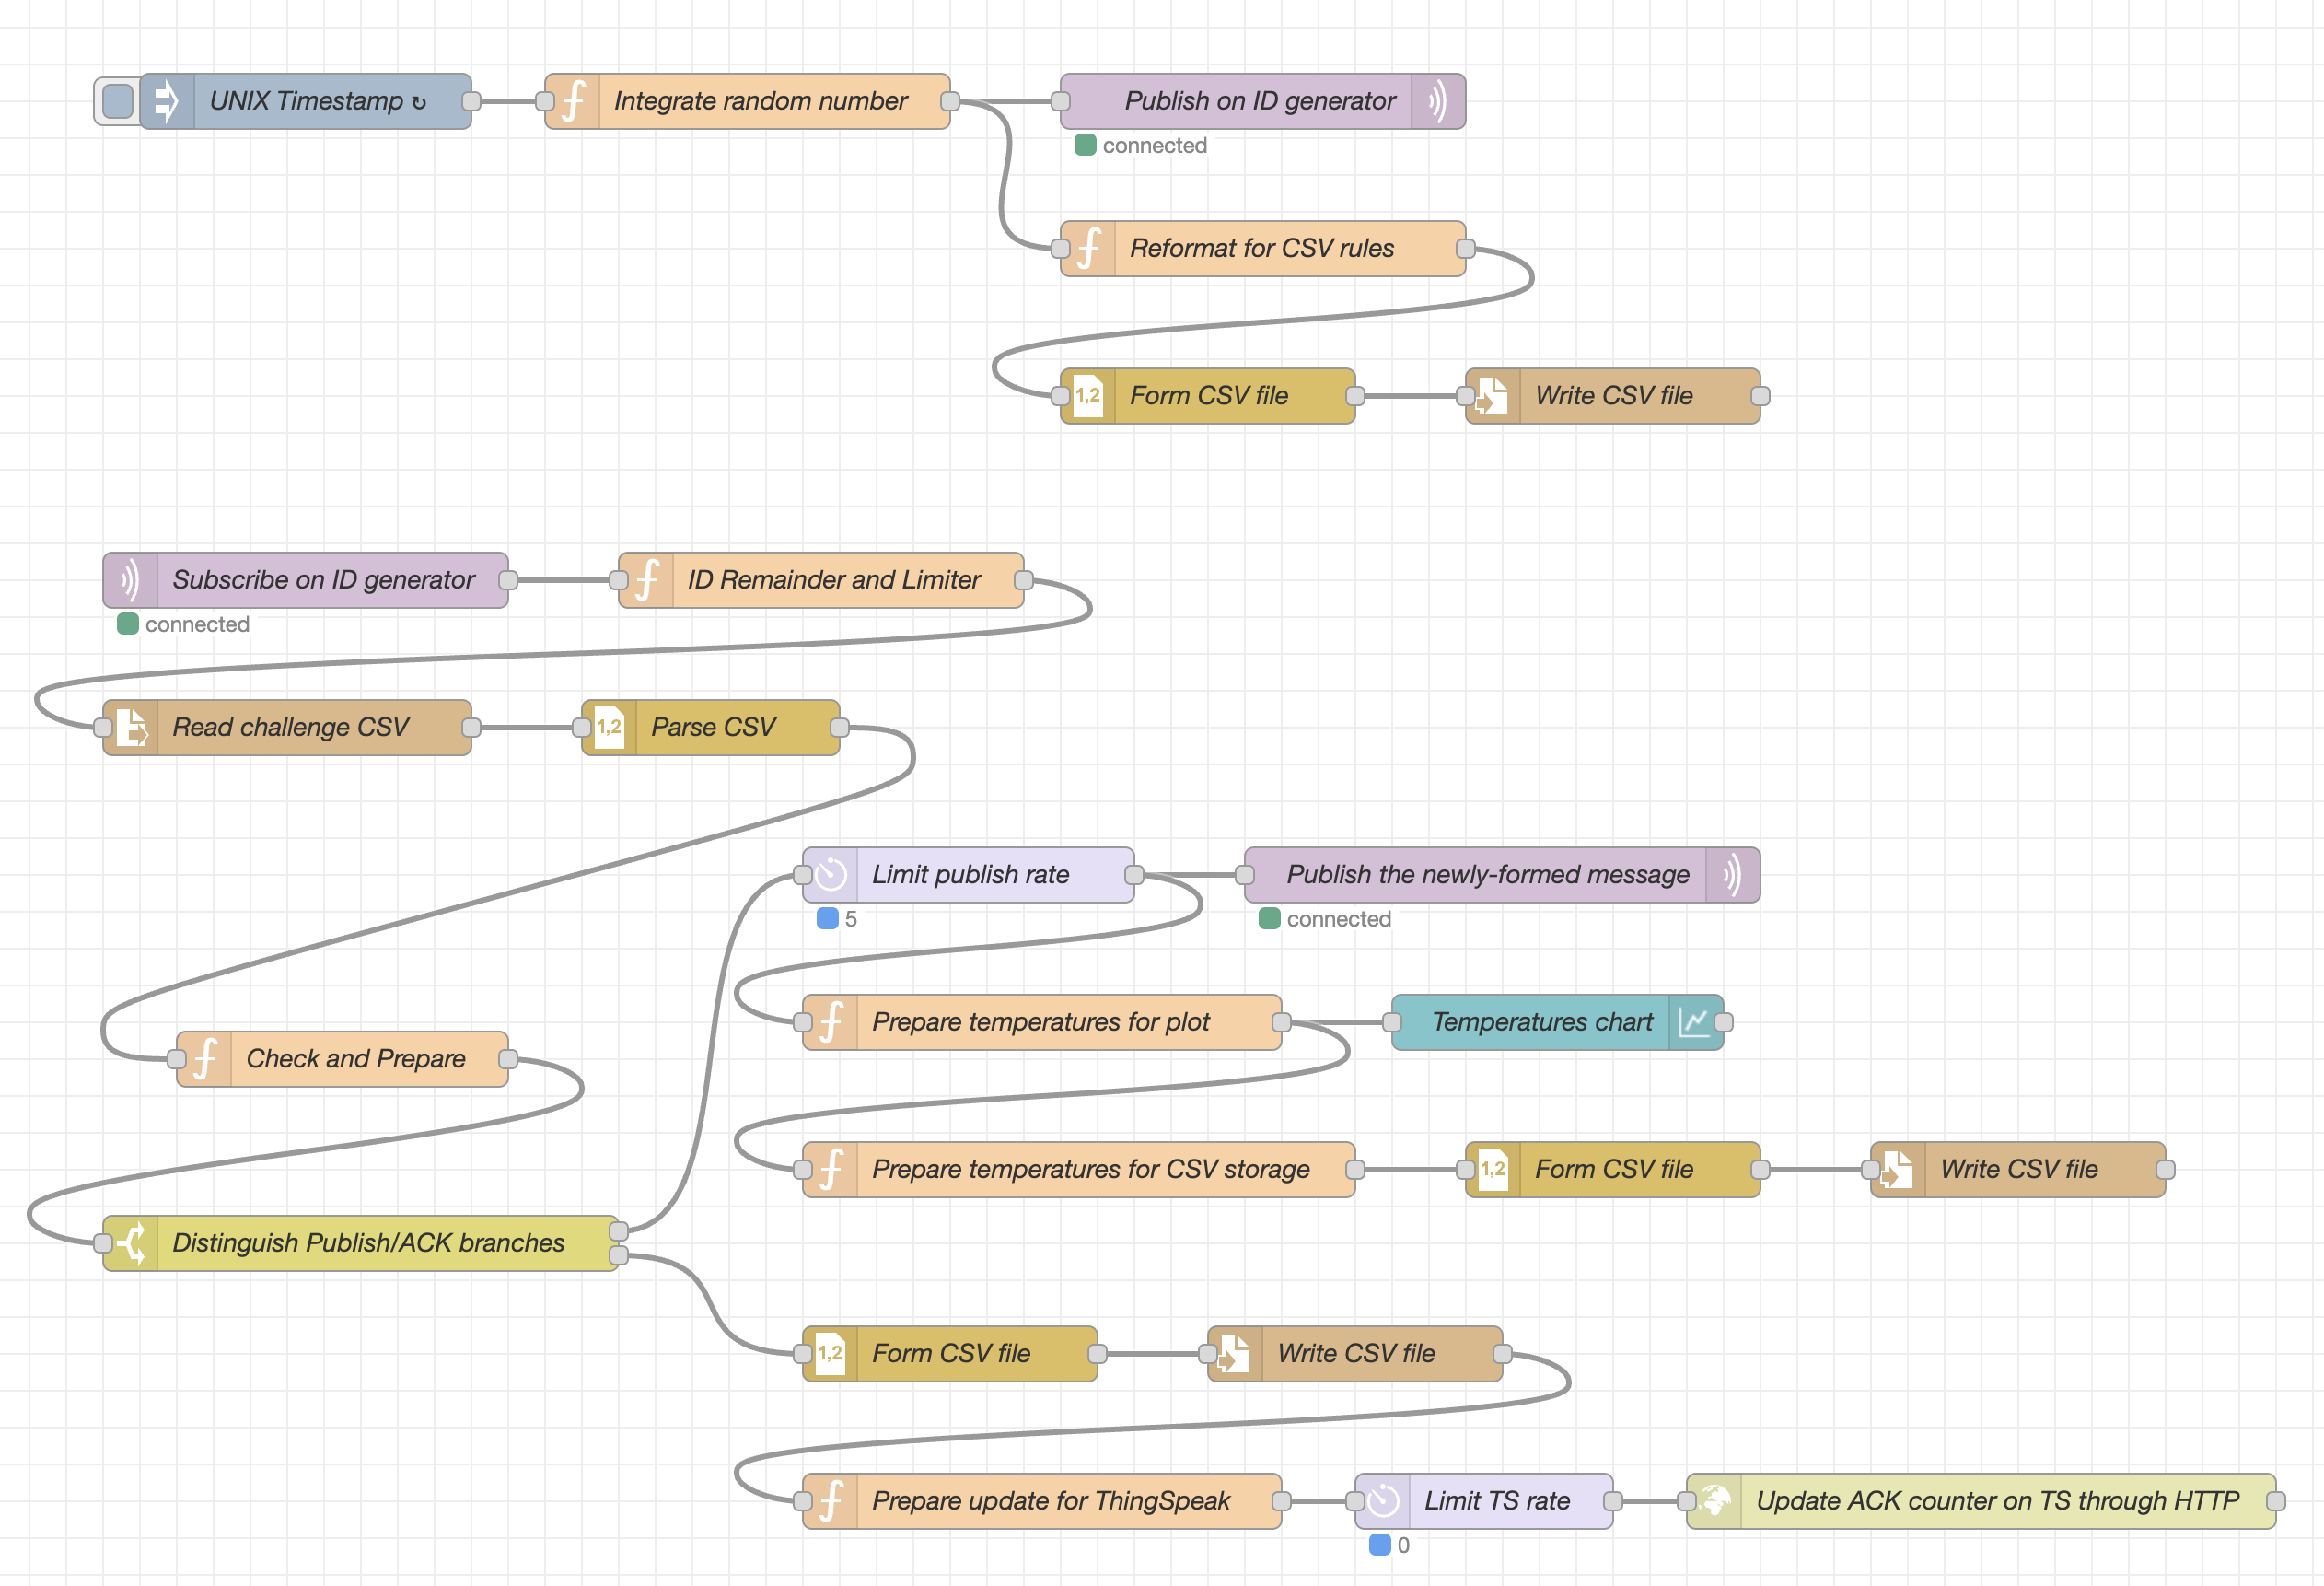
\includegraphics[width=18cm]{../res/node-red-chart}
    \end{center}

    \newpage

    \subsection*{ThingSpeak public channel}

    \href{https://thingspeak.mathworks.com/channels/2922298}{\texttt{https://thingspeak.mathworks.com/channels/2922298}}


    \section{Implementation and design choices}\label{sec:implementation-and-design-choices}

    All the question have been answered by implementing a \textsc{Node-RED} flow that integrates all the functionalities required by the first part of the Challenge, in a compact way, which eases readability and clarity of the overall structure.

    In the following description, each node has its own separate space, in which \textsc{Input}, \textsc{Output} and \textsc{Processing} details are provided.

    A deeper explaination of the most meaningful points is then expanded and correlated by the implementation of the \textsc{JavaScript function nodes}, when used.


    \section{ID Generator Publisher}\label{sec:id-generator-publisher}

    \subsection{UNIX Timestamp: injection node}\label{subsec:unix-timestamp:-injection-node}

    \subsubsection{Input}

    This is an injection node: no input is expected.

    \subsubsection{Output}

    \texttt{msg.timestamp} = current UNIX timestamp

    \medskip

    The current UNIX timestamp is the number of milliseconds elapsed from the Epoch (defined on 01/01/1970) and provides a relative time measurement of the instant in which the message has been generated.

    An example of the resulting output is provided in the following.

    \begin{minted}{JSON}
{
    "timestamp":1745243009801
}
    \end{minted}

    \subsubsection{Processing details}

    The processing phase is implicitly carried out by the node implementation.

    \subsection{Integrate random number: function node}\label{subsec:integrate-random-number:-function-node}

    \subsubsection{Input}

    The input is provided by the injection node, which generates a message containing the current UNIX timestamp, to integrate further.

    \subsubsection{Output}

    \texttt{msg.payload.timestamp} = UNIX timestamp,

    \texttt{msg.payload.id} = a random number between 0 and 30000 (included)

    \medskip

    Note that the resulting format is different from the one \hyperref[subsec:reformat-for-csv-rules:-function-node]{that will be later used for CSV storage}.

    \medskip

    An example of the resulting output is provided in the following.

    \begin{minted}{JSON}
{
    "payload":
        {
            "id":9026,
            "timestamp":1745243009801
        }
}
    \end{minted}

    \subsubsection{Processing details}

    The function node integrates the UNIX timestamp received in input with a random number between 0 and 30000 (included) that will then be used in \hyperref[subsec:check-and-prepare:-function-node]{successive computations}.

    \smallskip

    The payload is then formed aggregating both of them.

    \subsubsection{Implementation}

    \begin{minted}{JavaScript}
// Random generator boundaries
const RAND_MAX = 30000;
const RAND_MIN = 0;

// Integer random
let generated = Math.floor(Math.random() * RAND_MAX) + RAND_MIN;
let timestamp = msg.timestamp;

// Prepare the payload format of the MQTT Publish message
// Note this format is different from the one used in the CSV file, as per specifications
msg = {
    payload: {
        id: generated, // the generated integer random number
        timestamp: timestamp // the left parameter being the payload field, the right one being the local variable
    }
}

return msg;
    \end{minted}

    \subsection{Publish on ID Generator: MQTT Publisher node}\label{subsec:publish-on-id-generator:-mqtt-publisher-node}

    \subsubsection{Input}

    The aggregated \textsc{Publish Message} described \hyperref[subsec:integrate-random-number:-function-node]{earlier} is injected.

    \subsubsection{Output}

    This is a publish node: no output is expected.

    \subsubsection{Processing details}

    The aggregated payload is published on the \texttt{challenge3/id\_generator} topic, as per specifications.

    \smallskip

    All of the MQTT publishing parameters are statically set via the node parameters.

    \smallskip

    \textsc{QoS} and \textsc{Retain} values are set to their default (\textsc{0} and \textsc{False}, respectively).

    \subsection{Reformat for CSV rules: function node}\label{subsec:reformat-for-csv-rules:-function-node}

    \subsubsection{Input}

    The aggregated \textsc{Publish Message} described \hyperref[subsec:integrate-random-number:-function-node]{earlier} is injected.

    \subsubsection{Output}

    \texttt{msg.payload."No."} = sequential counter of published IDs,

    \texttt{msg.payload.ID} = the randomly generated ID,

    \texttt{msg.payload.TIMESTAMP} = the UNIX timestamp

    \medskip

    An example of the resulting output is provided in the following.

    \begin{minted}{JSON}
{
    "payload":
        {
            "No.":3,
            "ID":9026,
            "TIMESTAMP":1745243009801
        }
}
    \end{minted}

    \subsubsection{Processing details}

    The published values are moved to a convenient position for CSV parsing and respecting the specifications for CSV formatting.

    \smallskip

    A local context counter is stored and updated to integrate the payload fields with it.

    \smallskip

    In a sense, it also acts as a change node and formatter for the publishing parameters, integrating their roles via code.

    \subsubsection{Implementation}

    On node start (executed only once, at flow deployment):

    \begin{minted}{JavaScript}
// The ID counter starts from 0, as it is always incremented before usage
if (context.get("id_counter") === undefined) {
    context.set("id_counter", 0);
}
    \end{minted}

    On message arrival (standard function node behaviour):

    \begin{minted}{JavaScript}
// Increment the ID counter (from local node context)
context.set("id_counter", context.get("id_counter") + 1);

// Form the payload content with the parameters required by the CSV formatting
// Starting from the ones provided as part of the Publish payload
// In a sense, this function node also serves as a change node for the already provided parameters
// For the CSV parsing to happen, the interested fields must be present in the output payload
msg.payload = {
                "No.": context.get("id_counter"),
                ID: msg.payload.id,
                TIMESTAMP: msg.payload.timestamp
};

return msg;
    \end{minted}

    \subsection{Form CSV file: CSV formatting node}\label{subsec:form-csv-file:-csv-formatting-node}

    \subsubsection{Input}

    The re-formatted \textsc{Publish Message} is injected.

    \subsubsection{Output}

    \texttt{msg.payload} = CSV payload,

    \texttt{msg.columns} = CSV headers

    \medskip

    An example of the resulting output is provided in the following.

    \begin{minted}{JSON}
{
    "payload":"3,9026,1745243009801",
    "columns":"No.,ID,TIMESTAMP"
}
    \end{minted}

    \subsubsection{Processing details}

    The chosen line separators (Linux, \texttt{\textbackslash n}) are injected through the CSV formatting node and not via the \textsc{Write File} one, so they should not be repeated later.

    \smallskip

    Empty and null fields are included in the parsing procedure.

    \smallskip

    Headers are instead included only at flow deployment (so they behave as expected, being present only at the first line of the output file).

    \subsection{Write CSV file: file output node}\label{subsec:write-csv-file:-file-output-node}

    \subsubsection{Input}

    The CSV payload formatted for CSV output writing.

    \subsubsection{Output}

    The output of this node replicates the input, but integrates the file name on which the CSV payload is stored (\texttt{msg.filename = "/data/challenge/id\_log.csv"}).

    \smallskip

    On the machine's disk, of course, it also writes (and updates) the CSV output file.

    \subsubsection{Processing details}

    New content is, naturally, appended.

    \smallskip

    Line separators are already injected by the CSV parsing node (see \hyperref[subsec:reformat-for-csv-rules:-function-node]{related notes}).


    \section{ID Generator Subscriber and parser}\label{sec:id-generator-subscriber-and-parser}

    \subsection{Subscribe on ID generator: MQTT Subscriber node}\label{subsec:subscribe-on-id-generator:-mqtt-subscriber-node}

    \subsubsection{Input}

    This is a subscribe node: no input is expected.

    \subsubsection{Output}

    The received resulting \textsc{Publish Message} is returned.

    \smallskip

    The expected format, topic and parameters are the same \hyperref[sec:id-generator-publisher]{described at the \textsc{Publish} side}.

    \medskip

    An example of the resulting output is provided in the following.

    \begin{minted}{JSON}
{
    "topic":"challenge3/id_generator",
    "payload":
        {
            "id":28784,
            "timestamp":1745242246354
        },
    "qos":0,
    "retain":false
}
    \end{minted}

    \subsubsection{Processing details}

    The aggregated payload is received on the \texttt{challenge3/id\_generator} topic, as per specifications.

    \smallskip

    All of the MQTT subscribe parameters are statically set via the node parameters.

    \smallskip

    \textsc{QoS} value is set to its default (\textsc{0}).

    \subsection{ID Remainder and Limiter: function node}\label{subsec:id-remainder-and-limiter:-function-node}

    \subsubsection{Input}

    The received \textsc{Publish Message} by means of the ID generator subscription.

    \subsubsection{Output}

    The expected output matches the received \textsc{Publish Message}, integrates the remainder (via the modulo operation) and stores a copy of the \textsc{Publish} payload (\texttt{id} and \texttt{timestamp} values), for \hyperref[subsec:check-and-prepare:-function-node]{successive computations}.

    \smallskip

    \texttt{msg.remainder} = the result of the modulo operation,

    \texttt{msg.sub} = the received \textsc{Publish Message} by means of the subscription

    \medskip

    An example of the resulting output is provided in the following.

    \begin{minted}{JSON}

{
    "remainder":5651,
    "sub":
        {
            "id":28784,
            "timestamp":1745242246354
        }
}
    \end{minted}

    \subsubsection{Processing details}

    The ID process limit is implemented trough a local context counter, described in the following, alongside the remainder computation.

    \subsubsection{Implementation}

    On node start (executed only once, at flow deployment):

    \begin{minted}{JavaScript}
// The ID process counter starts from -1, as it is always incremented before usage
if (context.get("process_counter") === undefined) {
    context.set("process_counter", -1);
}
    \end{minted}

    On message arrival (standard function node behaviour):

    \begin{minted}{JavaScript}
const REMAINDER_NUM = 7711; // constant (number of CSV entries in the provided input file)
const ID_PROCESS_LIMIT = 80; // maximum number of subscription-side ID messages to process

let payload = msg.payload;

// Reset the message structure, for clarity
msg = {};
// Modulo operation
msg.remainder = parseInt(payload.id) % REMAINDER_NUM;
// Storage of the received subscription payload (it will be useful in the successive computation)
msg.sub = payload;

// The local processing counter is updated
context.set("process_counter", context.get("process_counter") + 1);

// Checks if the resulting message is 0 (not existing, since counting starts from 1 in the CSV file, but note that it is still counted in the process limit)
// or the processing counter has been reached and successive messages are to be discarded (no return)
if (msg.remainder !== 0 && context.get("process_counter") < ID_PROCESS_LIMIT) // <= if instead counting from 0
    return msg;
    \end{minted}

    \subsection{Read challenge CSV: file input node}\label{subsec:read-challenge-csv:-file-input-node}

    \subsubsection{Input}

    The integrated \textsc{Publish Message} flowing as part of the subscription.

    \smallskip

    In this case, it serves as an injection node, to let the activity of the file input read start (its fields will be replicated for successive computations).

    \subsubsection{Output}

    The unformatted input file, served as a complete flattened string, for \hyperref[subsec:parse-csv:-csv-formatting-node]{successive CSV parsing}, alonside the rest of the remainder and subscription fields, being replicated.

    \smallskip

    \texttt{msg.payload} = complete flattened CSV string

    \subsubsection{Processing details}

    The provided input file is read and returned as payload to the parser node.

    \subsection{Parse CSV: CSV formatting node}\label{subsec:parse-csv:-csv-formatting-node}

    \subsubsection{Input}

    The unformatted challenge CSV file, served as a complete flattened string, for CSV parsing.

    \subsubsection{Output}

    The CSV input payload formatted for JSON/JavaScript computations, as a JavaScript data structure.

    \medskip

    An example of the resulting output is provided in the following.

    \begin{minted}{JSON}
{
    "payload":"(omitted, the resulting array containing all the parsed messages)",
    "remainder":5651,
    "sub":{
        "id":28784,
        "timestamp":1745242246354
    },
    "filename":"/data/challenge/challenge3.csv",
    "columns":"No.,Time,Source,Destination,Protocol,Length,Source Port,Destination Port,Info,Payload"
}
    \end{minted}

    \subsubsection{Processing details}

    Empty and null fields are included in the parsing procedure.

    \subsection{Check and Prepare: function node}\label{subsec:check-and-prepare:-function-node}

    \subsubsection{Input}

    The CSV input payload formatted for JSON/JavaScript computations, as a JavaScript data structure.

    \subsubsection{Output}

    A \textsc{Publish Message}, which is then eventually re-formatted for temperature analysis or an \textsc{Acknowledgement Message}.

    \smallskip

    They are \hyperref[subsec:distinguish-publish/ack-branches:-switch-node]{later distinguished by a \textsc{Switch} node}.

    \medskip

    An example of the resulting output is provided in the following.

    \medskip

    A \textsc{Publish Message}:

    \begin{minted}{JSON}
{
    "topic":"factory/room1/room6/hydraulic_valve",
    "payload":
        {
            "timestamp":1745249897928,
            "id":27562,
            "topic":"factory/room1/room6/hydraulic_valve",
            "payload":{
                "unit": "F",
                "long": 87,
                "description": "Room Temperature",
                "lat": 91,
                "range": [10, 37],
                "type": "temperature"
            }
        }
}
    \end{minted}

    \smallskip

    An \textsc{Acknowledgement Message}:

    \begin{minted}{JSON}
{
    "payload":
        {
            "No.":12,
            "TIMESTAMP":1745259353585,
            "SUB_ID":296,
            "MSG_TYPE":"Publish Ack"
        }
}
    \end{minted}

    \subsubsection{Processing details}

    In the provided CSV, numbering starts from 1, unlike JavaScript data structures, that are instead numbered starting from 0: the input reimainder is adapted to the CSV format.

    \smallskip

    Packets that apply the \textsc{Piggy-Backing} technique (transporting more than one description and payload in their structure) are assumed to have a well-formed separation architecture.

    \smallskip

    The number of descriptions and related payloads are therefore assumed to be the same, but can be null or not validly defined.

    \smallskip

    The edge case, in which an aggregated message carries disomogeneous types (therefore disaligning payloads indexes) is also managed, through a support counter for any other kind of message type encountered.

    \smallskip

    A FIFO data structure, in the form of a Stack, is used to form a network buffer that stores the packets that will be returned by the node.

    \smallskip

    \textsc{JSON} parsing is then applied to the remaining fields, in a coherent format with respect to the specifications.

    \smallskip

    In \textsc{Node-RED}, there are two possible strategies implementing a network buffer:

    \begin{itemize}
        \item Flattening: An arbitrarily complex and convoluted data structure is flattened in output, multiplying the number of returned messages by the cardinality of the data structure used.

        The implementing syntax requires indication of the interested data structure between brackets: \texttt{return [buffer];}.

        This is the chosen approach.
        \item Pull-based: A FIFO data structure is enforced: in the buffering node, messages are pushed, while in the receiving node, messages are pulled singularly.

        This is an unnatural approach in \texsc{Node-RED}, being it based on a continuous message flow, that is clearly represented by its implementation chart.
    \end{itemize}

    \subsubsection{Implementation}

    On node start (executed only once, at flow deployment):

    \begin{minted}{JavaScript}
// The global ACK counter starts from 0, as it is always incremented before usage
// Specifications require the global counter is reset at each flow deployment
// This code will be executed only once, when deploying/updating the flow
global.set("ack_counter", 0);
    \end{minted}

    On message arrival (standard function node behaviour):

    \begin{minted}{JavaScript}
// The input flowing in the function node is the output of the CSV read-file parsing
let csv_entries = msg.payload;
// In the provided CSV, numbering starts from 1, unlike JavaScript data structures that are numbered from 0
// As described earlier, this motivates the exclusion of the remainder 0 by dropping a possible resulting packet
let remainder = msg.remainder - 1;

// Parsing of the packet description (type of packet)
// Packets applying piggy-backing (transporting more than one description+payload in their structure)
// are separated by a comma (,) and a space ( )
// This produces an array data structure in which each packet information and payload is separated
let info = String(csv_entries[remainder].Info);
let infos = info.split(", ");

// Parsing of the packet payload
// Packets applying piggy-backing (transporting more than one description+payload in their structure)
// are separated by a comma (,) and a curly bracket ({)
// This produces an array data structure in which each packet information and payload is separated
// The curly bracket ({) is restored back since it is already part of the JSON payload inner structure
let payload = String(csv_entries[remainder].Payload);
let payloads = payload.split(",{");
for (let i = 1; i < payloads.length; i++)
    payloads[i] = '{' + payloads[i];

// A Publish Message has its own description separated by the topic through a couple of brackets (Publish Message (eventual id) [topic])
// Therefore, the interesting part for identification is before the opening bracket ([), translating to the first position of the split result
let types = [];
for (let i = 0; i < infos.length; i++)
    types[i] = infos[i].split(' [')[0];

// Explicit assertion: the number of packet descriptions and payloads is the same.
// A payload being null or undefined still passes this check (being it still a payload, but with a non-meaningful value).
// A non formatted payload in a piggy-backed message (containing more than one) can't be incoherent in size.
// The case in which the number of descriptions does not match the number of payloads is therefore not valid, in an unformatted environment.
// Instead, the case in which the message is well formatted but one or more payloads (or its components)
// are missing is coherent and valid parsing is performed in the following.
let publish_checker = 0;
types.forEach(t => {
    if (t.startsWith("Publish Message"))
        publish_checker++;
});
console.assert(publish_checker == payloads.length);

// A support variable, used to gather the right payload match later
let non_publish_counter = 0;

// A Stack (FIFO) data structure, acting as a network buffer
// Its behaviour is ideal both for the flattening and FIFO cases (see notes)
let buffer = [];
for (let i = 0; i < infos.length; i++) {
    let type = types[i];
    // As shown, a publish message is declared with "Publish Message" at the beginning of its description
    if (type.startsWith('Publish Message')) {
        // Publish Messages are of course interleaved with any other piggy-backed message, potentially not being a Publish one
        // (and therefore not carrying a payload)
        payload = payloads[i - non_publish_counter];
        // As described earlier, the next part of the split result is now interesting for the topic identification
        // Next, it is also split for the closing bracket (]) being the separator for the topic identifier ending
        let topic = infos[i].split('[')[1].split(']')[0];
        // manage the case of null or undefined payload
        if (payload === null || payload === undefined || payload.length === 0) {
            payload = "{}"; // replace with empty JSON payload, as per specifications
        }

        // Final publishing content setup, as per specifications
        let content = {
            timestamp: Date.now(), // UNIX timestamp (number of milliseconds elapsed from the standard Epoch time discriminant (01/01/1970))
            id: msg.sub.id, // ID of the message received through the ID generator subscription (see previous description)
            topic: topic, // Identified topic
            payload: payload // n-th payload in the message
        }

        let result = {
            topic: topic, // the MQTT topic on which to publish can also be set via the topic property
            // But must be replicated in this field, since is required by the MQTT Publisher node to operate correctly
            payload: content // Content described earlier
        }

        // FIFO data structure behaviour: the resulting publish message is pushed
        // to be popped by successive computations
        buffer.push(result);
    } else if (type.includes('Ack')) {
        non_publish_counter++;
        // The global ACK counter is updated among (possibly) the whole Node-RED installation
        global.set("ack_counter", global.get("ack_counter") + 1);

        // Final ACK content setup, as per specifications
        // The chosen format is already the one that will be parsed and stored in the CSV file
        let content = {
            "No.": global.get("ack_counter"), // Global ACK counter (can be seen by the whole installation)
            TIMESTAMP: Date.now(), // UNIX timestamp (number of milliseconds elapsed from the standard Epoch time discriminant (01/01/1970))
            SUB_ID: msg.sub.id, // ID of the message received through the ID generator subscription (see previous description)
            // An Acknowledgement message has its own description separated by the ID through a couple of brackets (Publish Ack (eventual id) [eventual notes])
            // Therefore, the interesting part for identification is before the opening bracket ((), translating to the first position of the split result
            // Then, it must be separated by the following opening bracket ([) for notes
            MSG_TYPE: (type.split(' (')[0]).split('[')[0]
        }

        let result = {
            // ACKs, of course, do not have a topic, as they will not be published!
            // This is a sufficient characteristic to let the Switch node differentiate among the two message kinds!
            payload: content
        }

        // FIFO data structure behaviour: the resulting publish message is pushed
        // to be popped by successive computations
        buffer.push(result);
    } else non_publish_counter++;
}

// Node-RED operates flattening on the return structure,
// so there will be separate messages being returned for both single and piggy-backed aggregated messages
return [buffer];
    \end{minted}

    \subsection{Distinguish Publish/ACK branches: switch node}\label{subsec:distinguish-publish/ack-branches:-switch-node}

    \subsubsection{Input}

    The aggregated data structure carrying a \textsc{Publish} or an \textsc{Acknowledgement} message, for \hyperref[subsec:prepare-temperatures-for-csv-storage:-function-and-csv-formatting-node]{later analysis}.

    \subsubsection{Output}

    The input message is replicated on the chosen branch.

    \subsubsection{Processing details}

    Uses the topic presence as a discriminant among \textsc{Publish} and \textsc{Acknowledgement} messages.

    \smallskip

    The processing flow continues in two separate output branches.

    \subsection{Publish the newly-formed message: MQTT Publisher node}\label{subsec:publish-the-newly-formed-message:-mqtt-publisher-node}

    \subsubsection{Input}

    The aggregated \textsc{Publish Message} formed by the function node is retrieved from the FIFO buffer (in our case, automatically flattened by \textsc{Node-RED}).

    \smallskip

    It is filtered by a rate limiter node, that, per specifications, is set to a limit of 4 messages per minute.

    \subsubsection{Output}

    This is a publish node: no output is expected.

    \subsubsection{Processing details}

    Reliability MQTT publishing parameters are statically set via the node parameters.

    \smallskip

    The topic used is the one received by the \textsc{Publish Message}, as per specifications (therefore, it is dynamic).

    \smallskip

    \textsc{QoS} and \textsc{Retain} values are set to their default values (\textsc{0} and \textsc{False}, respectively).

    \subsection{Prepare temperatures for plot: function node}\label{subsec:prepare-temperatures-for-plot:-function-node}

    \subsubsection{Input}

    The aggregated \textsc{Publish Message} formed by the function node is retrieved from the FIFO buffer (in our case, automatically flattened by \textsc{Node-RED}).

    \smallskip

    It is filtered by a rate limiter node, that, per specifications, is set to a limit of 4 messages per minute.

    \subsubsection{Output}

    The average temperature measured by the input message range, alongside the parsed message.

    \smallskip

    The payload (average temperature measured) is used to draw the temperatures chart.

    \smallskip

    It is then available through the \textsc{Node-RED Dashboard} (at \texttt{/ui}).

    \smallskip

    \texttt{msg.payload} = average temperature measurement,

    \texttt{msg.parsed} = JSON parsed message payload

    \medskip

    An example of the resulting output is provided in the following.

    \begin{minted}{JSON}
{
    "payload":23.5,
    "parsed":
        {
            "description":"Room Temperature",
            "long":87,
            "range":[10, 37],
            "lat":91,
            "type":"temperature",
            "unit":"F"
        }
}
    \end{minted}

    \subsubsection{Processing details}

    Some parsing checks are needed when filtering out unparsable or incomplete payloads.

    \smallskip

    Moreover, some explicit assumptions need to be checked: payload type is \texttt{temperature} and unit is \texttt{F} (Fahrenheit).

    \smallskip

    The range is also composed by exactly 2 (possibly floating-point) numbers that are then parsed when computing the final average value.

    \smallskip

    \subsubsection{Implementation}

    \begin{minted}{JavaScript}
let parsed;

// The payload received through the published message is parsed.
// If no parsing is possible (the payload is therefore invalid),
// the payload is nulled and the whole message discarded by the successive check
try {
    parsed = JSON.parse(msg.payload.payload);
} catch (e) { parsed = null; }

if (parsed !== null && // the parsed payload is null or converted to null being it unparsable
    parsed !== undefined && // the parsed payload, even if parsed, has no useful content detected
    parsed.type === "temperature" && // the message being transported is a temperature measurement
    parsed.unit === "F" && // the used unit is Fahrenheit degrees
    parsed.range !== null && // the temperature range is invalid or empty
    parsed.range !== undefined &&
    parsed.range.length === 2) { // temperature range is (as expected) composed by both the minimum and maximum values

    let range = {
        min: parseFloat(parsed.range[0]), // the minimum value is the first part of the range
        max: parseFloat(parsed.range[1]) // the maximum value is the second part of the range
    };

    // The range is prepared for plotting
    let ret = {
        // Average calculation
        payload: (range.min + range.max) / 2,
        // Storage of the parsed payload for successive computations
        parsed: parsed
    }

    return ret;
}
    \end{minted}

    \subsubsection{Temperatures chart: example of resulting plot}

    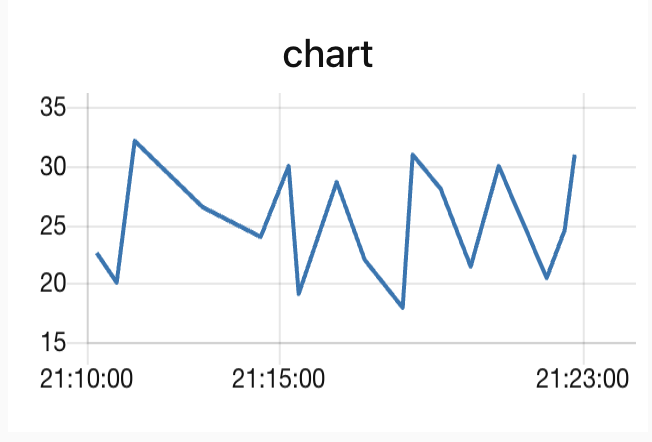
\includegraphics[height=5cm]{../res/temperatures-chart}

    \subsection{Prepare temperatures for CSV storage: function and CSV formatting node}\label{subsec:prepare-temperatures-for-csv-storage:-function-and-csv-formatting-node}

    \subsubsection{Input}

    The parsed JSON message, with all its fields and the computed temperature average.

    \subsubsection{Output}

    \texttt{msg.payload} = CSV-formatted fields (\texttt{No.,LONG,LAT,MEAN\_VALUE,TYPE,UNIT,DESCRIPTION})

    \medskip

    An example of the resulting output is provided in the following.

    \begin{minted}{JSON}
{
    "payload":
        {
            "No.":1,
            "LONG":87,
            "LAT":91,
            "MEAN_VALUE":23.5,
            "TYPE":"temperature",
            "UNIT":"F",
            "DESCRIPTION":"Room Temperature"
        }
}
    \end{minted}

    \subsubsection{Processing details}

    The temperatures counter is a local node context variable, updated before usage and prepared at flow initialization.

    \smallskip

    The CSV-formatted style is then prepared gathering all of the parsed parameters.

    \subsubsection{Implementation}

    On node start (executed only once, at flow deployment):

    \begin{minted}{JavaScript}
// The stored temperatures counter starts from 0, as it is always incremented before usage
if (context.get("temp_counter") === undefined) {
    context.set("temp_counter", 0);
}
    \end{minted}

    On message arrival (standard function node behaviour):

    \begin{minted}{JavaScript}
// The stored temperatures counter is incremented before usage
context.set("temp_counter", context.get("temp_counter") + 1);

// The parsed payload has been piggy-backed earlier by the input node
let parsed = msg.parsed;
// The average temperature value has been set as payload for plot display
let mean = msg.payload;

msg = {};

msg.payload = {
                "No.": context.get("temp_counter"), // Stored temperatures counter
                LONG: parsed.long, // Longitude
                LAT: parsed.lat, // Latitude
                MEAN_VALUE: mean, // Average temperature
                TYPE: parsed.type, // Expected type is "temperature" (measurement)
                UNIT: parsed.unit, // Expected unit is "F" (Fahrenheit)
                DESCRIPTION: parsed.description // A description of the payload content
};

return msg;
    \end{minted}

    \subsection{Prepare update for ThingSpeak: function node}\label{subsec:prepare-update-for-thingspeak:-function-node}

    \subsubsection{Input}

    The CSV-parsed \textsc{Acknowledgement} structure is provided to the function node after storage.

    \smallskip

    Its format has already been \hyperref[subsec:check-and-prepare:-function-node]{defined earlier}, when preparing for branching, and is not modified after, since its only usage destinations are compatible with the former format style.

    \subsubsection{Output}

    An \textsc{HTTP Request} is built up imposing the \textsc{GET} method and the \textsc{ThingSpeak} API Writing Endpoint \textsc{URL}, correlated by the private \textsc{API Key} and updated global \textsc{Acknowledgement} counter.

    \smallskip

    It is then filtered by a rate limiter node, imposing a message limit of one per 20-second period, as per ThingSpeak free plan requirements.

    \smallskip

    \texttt{msg.method} = the \textsc{HTTP Request} method (GET),

    \texttt{msg.url} = the \textsc{ThingSpeak} API Writing Endpoint URL, appended to the \textsc{API Key} and updated global ACK counter value

    \medskip

    An example of the resulting output is provided in the following.

    \begin{minted}{JSON}
{
    "method":"GET",
    "url":"https://api.thingspeak.com/update?api_key=API_KEY&field1=4"
}
    \end{minted}

    \subsubsection{Processing details}

    Messages flowing outside the rate limit are queued.

    \smallskip

    The global \textsc{Acknowledgement} counter is stored for the whole \textsc{Node-RED} installation while active.

    \subsubsection{Implementation}

    \begin{minted}{JavaScript}
// The API Key is stored as a local node variable and used as part of the URL contacted through HTTP
let API_KEY = "<omitted>";

msg = {};
msg.method = "GET";
// A GET request to the ThingSpeak API endpoint for data writes is prepared, packing up also the global ACK counter
msg.url = "https://api.thingspeak.com/update?api_key=" + API_KEY + "&field1=" + global.get("ack_counter");

return msg;
    \end{minted}
\end{document}